\documentclass[xelatex,12pt]{beamer}
\usepackage{pgfpages}
\usepackage{fontspec}
\usepackage{xunicode}
\usepackage{polyglossia}
\PolyglossiaSetup{french}{indentfirst=false}
\usepackage[french=guillemets]{csquotes}
\usepackage{xpatch}
\usepackage{diagbox}

\setmainlanguage{french}
\xapptocmd\ttfamily{\XeTeXinterchartokenstate=0 }{}{}
\newcommand{\nospace}[1]{\texttt{#1}}

\usepackage{algorithm}
\usepackage[noend]{algpseudocode}
    \newcounter{lastenum}
    \newcommand{\mtpause}{\setcounter{lastenum}{\value{enumi}}}
    \newcommand{\mtresume}{\setcounter{enumi}{\value{lastenum}}}
\resetcounteronoverlays{lastenum}

\usepackage[backend=biber, style=chem-acs]{biblatex}
\addbibresource{Modele.bib} 
\setbeamertemplate{bibliography item}[triangle]


 
\usepackage{multirow}% row fusion
\usepackage{array} % column fusion
\usepackage{xfrac} % small fractions
\usepackage{adjustbox}
\usepackage{listings}

\usepackage{color}
\definecolor{gray}{rgb}{0.4,0.4,0.4}
\definecolor{darkblue}{rgb}{0.0,0.0,0.6}
\definecolor{cyan}{rgb}{0.0,0.6,0.6}

\usetheme{Warsaw}

\setbeamertemplate{frametitle}{\nointerlineskip  
    \begin{beamercolorbox}[wd=\paperwidth,ht=2.75ex,dp=1.375ex]{frametitle}
        \hspace*{2ex}\insertframetitle \hfill {\small\insertframenumber/\inserttotalframenumber} \hspace*{1ex}%
    \end{beamercolorbox}}

\usecolortheme{wolverine}

\setbeameroption{hide notes} % Only slides
%\setbeameroption{show only notes} % Only notes
%\setbeameroption{show notes on second screen=right} % Both

 \titlegraphic{\vspace{-1cm}
      
\includegraphics[width=2.5cm]{images/logo_paris_8.png}\hspace*{4.75cm}~%
      \hfill
      
\includegraphics[width=2.5cm]{images/logo_junglebike.png}
}

 
\title{Système de Recommandation }
\subtitle{Apprentissage chez Junglebike}
\author[\textsc{Komlan DANTODJI}]{\textsc{Komlan Jean-Marie DANTODJI}}
\institute{\normalsize Université Paris 8, LIASD\\
Encadrante : Mme Rakia JAZIRI\\
Tutrice : Mme Alice Battarel
}
 
\beamertemplatenavigationsymbolsempty
\setbeamertemplate{blocks}[rounded][shadow=true]
\setbeamerfont{page number in head/foot}{size=\large}

\begin{document}
{ \setbeamertemplate{headline}{}
  \setbeamertemplate{footline}{}
  \begin{frame}
  \titlepage
  \end{frame}

\note{
}
}

\begin{frame}{Plan}
  \tableofcontents[sectionstyle=show/show, hidesubsections]
\note{
}  
\end{frame}

\section{Introduction}
\subsection{Présentation de l'entreprise}
\begin{frame}{JungleBike}
\begin{itemize}
		\item Start Up de B2C.
		\item Spécialisée dans le secteur du Vélo. 
		\item Une entreprise de E-commerce dans la vente de matériels de vélos dans le but de faciliter la réparation.
		\item Elle est fondée en 2018, le site e-commerce a été mis en ligne en 2020.
		\item Plus d'une vingtaine de fournisseur aujourd'hui.
\end{itemize}
\end{frame}

\subsection{Solutions proposées}
\begin{frame}{Solutions proposées}
\begin{itemize}
		\item Mise en ligne des matériels de vélos,
		\item Enregistrement du vélo permettant d’identifier le modèle et ses différentes pièces afin de faciliter la réparation,
		\item Mise en relation des clients avec les réparateurs.
\end{itemize}
\end{frame}

\begin{frame}{Processus de mise en ligne des produits}
\begin{figure}[H]
    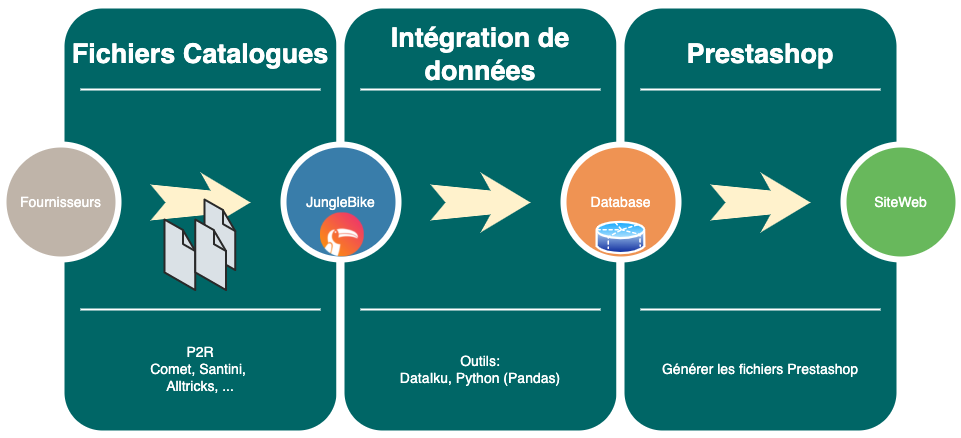
\includegraphics[width=11cm,height=4.8cm]{images/integration_steps.png}
    \caption{Processus de mise en ligne}
    \label{fig:L1}
\end{figure}
\end{frame}

\section{Contexte} % pour l'exposé final, commenter
%\subsection{Contexte} % pour l'exposé final, décommenter

\begin{frame}{Contexte RH}
  \begin{itemize}
  \item Equipe Data 
  \item Formé de deux data scientistes
  \item Intégration de donnée
  \item Construction des algoritmes de catégorisation et d'extration de données.
  \item Construcition des modèles de recommandation et d'analyse de sentiments.
  \end{itemize}
\end{frame}

\begin{frame}{Contexte technique}
  \begin{itemize}
  \item Outils: DataIku, DBeaver, .
  \item Langages et librairies: Python, Scikit Learn, Keras
  \end{itemize}
\end{frame}

\section{Problématique}

\subsection{Objectif}

\begin{frame}{Problème}
  \begin{itemize}
  \item Recommandation des produits basée sur les votes et le contenu des produits.
  \item Analyse du sentiment des clients basé sur les commentaires des clients sur les produits.
  \end{itemize}
\end{frame}

\subsection{Données}
\begin{frame}{Variables du jeu de donnée}
\begin{figure}[H]
    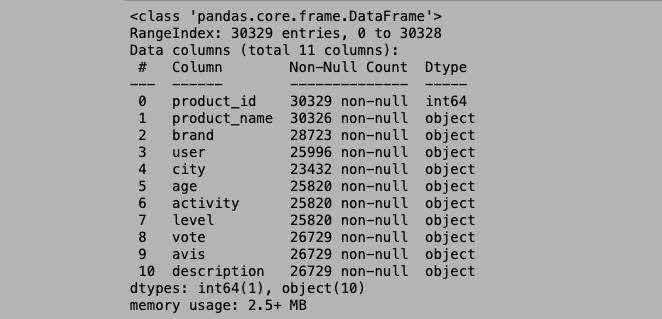
\includegraphics[width=11cm,height=4.8cm]{images/features.jpeg}
    \caption{ Transactions considérées}
    \label{fig:L1}
\end{figure}
\end{frame}
\begin{frame}{Données taille}
  \begin{itemize}
  \item 30.329 lignes, 11 colonnes
  \item Données récupérées par scrapping des sites des fournisseurs 
  \end{itemize}
\end{frame}

\begin{frame}{Aperçu du jeu de données}
\begin{figure}[H]
    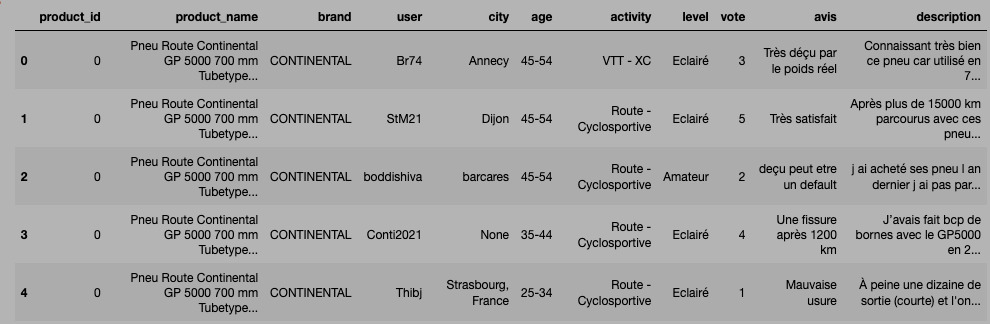
\includegraphics[width=11cm,height=4.8cm]{images/sample_data.jpeg}
    \caption{ Transactions considérées}
    \label{fig:L1}
\end{figure}
\end{frame} 


\section{État de l'art}
\subsection{Catégories d'algorithmes utilisés}
\begin{frame}{Catégories d'algorithmes utilisés}
  \begin{itemize}
  \item Recommandation basée sur le Contenu: Cosine Similarity
  \item Filtrage Collaboratif: Neural Collaborative Filtering
  \item Combinaison des deux premières
  \end{itemize}
\end{frame}

\subsection{Cosine Similarity}
\begin{frame}{Cosine Similarity}
	\begin{figure}[H]
    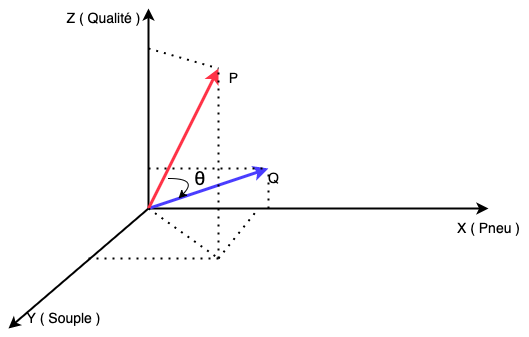
\includegraphics[width=\linewidth, height=4.8cm]{images/cosin_similarity.png}
    \caption{Détermination de l’hyperplan}
    \label{fig:L1}
\end{figure}
\end{frame}
\begin{frame}{Calcul du Cosine Similarity}
$${\text{cosine similarity}}=S_{C}(P,Q):=\cos(\theta )={\mathbf {P} \cdot \mathbf {Q}  \over \|\mathbf {P} \|\|\mathbf {Q} \|} $$
$$\cos(\theta ) ={\frac {\sum \limits _{i=1}^{n}{P_{i}Q_{i}}}{{\sqrt {\sum \limits _{i=1}^{n}{P_{i}^{2}}}}{\sqrt {\sum \limits _{i=1}^{n}{Q_{i}^{2}}}}}}$$

\end{frame}

%\section{Résultats obtenus}

\section{Conclusion}
  \begin{frame}{Conclusion}
  \begin{itemize}
		\item Beaucoup de travail d'intégration de donnée
		\item Prochainement je commence l'implémentation des algorithmes
\end{itemize}
  \end{frame}

% éléments hors section
\begin{frame}
\frametitle{Références}
\begin{thebibliography}{9}
\bibitem{texbook}
D Gunawan et al. The Implementation of Cosine Similarity to Calculate Text Relevance
between Two Documents. 2018 J. Phys.: Conf. Ser. 978 012120


\bibitem{lamport94}
Chakrabarti S, van den Berg M, Dom B 1999 Focused crawling: a new approach to topic-specific 
Web resource discovery Comput. Networks 31 11–16 pp 1623–1640 
\end{thebibliography}
\end{frame}



\begin{frame}
  \begin{block}{}
  \centering
  Merci pour votre attention
  \end{block}
\end{frame}


\end{document}
